\documentclass{extreport}

\usepackage[14pt]{extsizes}
\usepackage[T2A]{fontenc}
\usepackage[utf8]{inputenc}
\usepackage[english,ukrainian]{babel}

\usepackage[a4paper, top=10mm, bottom=15mm, left=20mm, right=15mm]{geometry}
\usepackage{amsmath,amsfonts,amssymb,amsthm,mathtools}
\usepackage{listings}
\usepackage{graphicx}
\usepackage{enumitem}
\usepackage{verbatim}
\usepackage{listings}
\usepackage{xcolor}
\usepackage{textgreek}
\usepackage{diagbox}
\usepackage{pgfplots}
\pgfplotsset{compat = 1.17}


\lstdefinestyle{output_txt}{
    basicstyle=\ttfamily\footnotesize,
    breakatwhitespace=false,         
    breaklines=true,                 
    captionpos=b,                    
    keepspaces=true,                                    
    numbersep=5pt,                  
    showspaces=false,                
    showstringspaces=false,
    showtabs=false,                  
    tabsize=2
}
\definecolor{codegreen}{rgb}{0,0.6,0}
\definecolor{codegray}{rgb}{0.5,0.5,0.5}
\definecolor{codepurple}{rgb}{0.58,0,0.82}
\lstdefinestyle{python_code}{ 
    commentstyle=\color{codegreen},
    keywordstyle=\color{magenta},
    numberstyle=\tiny\color{codegray},
    stringstyle=\color{codepurple},
    basicstyle=\ttfamily\footnotesize,
    breakatwhitespace=false,         
    breaklines=true,                 
    captionpos=b,                    
    keepspaces=true,                            
    numbersep=5pt,                  
    showspaces=false,                
    showstringspaces=false,
    showtabs=false,                  
    tabsize=4
}

\setlist[enumerate]{nosep}
\graphicspath{{pics/}}
\DeclareGraphicsExtensions{.png}

\begin{document}
\begin{titlepage}
    \thispagestyle{empty}
    \begin{center}
        
\includegraphics[width = \textwidth]{kpi}
        Міністерство освіти і науки України\\
        Національний технічний університет України\\
        <<Київський політехнічний інститут ім. І. Сікорського>>\\
        Інститут прикладного системного аналізу
    \end{center}
    \vspace{40mm}
    \begin{center}
        \textbf{Лабораторна робота} \\
        з курсу <<Методи оптимізації>> \\
        з теми <<Чисельні методи безумовної оптимізації першого порядку. 
        Градієнтний метод та його варіації>>
    \end{center}
    \vspace{20mm}
    \begin{flushleft}
        Виконали студенти 3 курсу групи КА-81 \\
        Галганов Олексій \\
        Єрко Андрій \\
        Фордуй Нікіта
    \end{flushleft}
    \begin{flushright}
        Перевірили \\
        Спекторський Ігор Якович \\
        Яковлева Алла Петрівна
    \end{flushright}
    \vspace{30mm}
    \begin{center}
        \textbf{Київ 2021}
    \end{center}
\end{titlepage}

\begin{center}
    \textbf{Варіант 1}
\end{center}
\textbf{Завдання.} Скласти програму для мінімізації цільової функції
одним з градієнтних методів. Конкретний тип градієнтного методу обрати
самостійно, ураховуючи особливості цільової функції.

\emph{Цільова функція:}
$f(x,y) = x^2 + 18y^2 + 0.01xy + x - y$

\noindent\textbf{Результати роботи.}
Для визначення опуклості цільової функції розглянемо її матрицю Гессе
$f''(x,y) = \begin{pmatrix}
    2 & 0.01 \\
    0.01 & 36
\end{pmatrix}$. Її власні числа приблизно рівні 2 та 36, 
тому цільова функція є строго опуклою. До того ж,
відношення власних чисел рівне $1/18$, тому лінії рівня
функції будуть видовженими еліпсами.
Також це видно з графіку цільової функції та її ліній рівня.
\begin{center}
    \begin{tabular}{c c}
        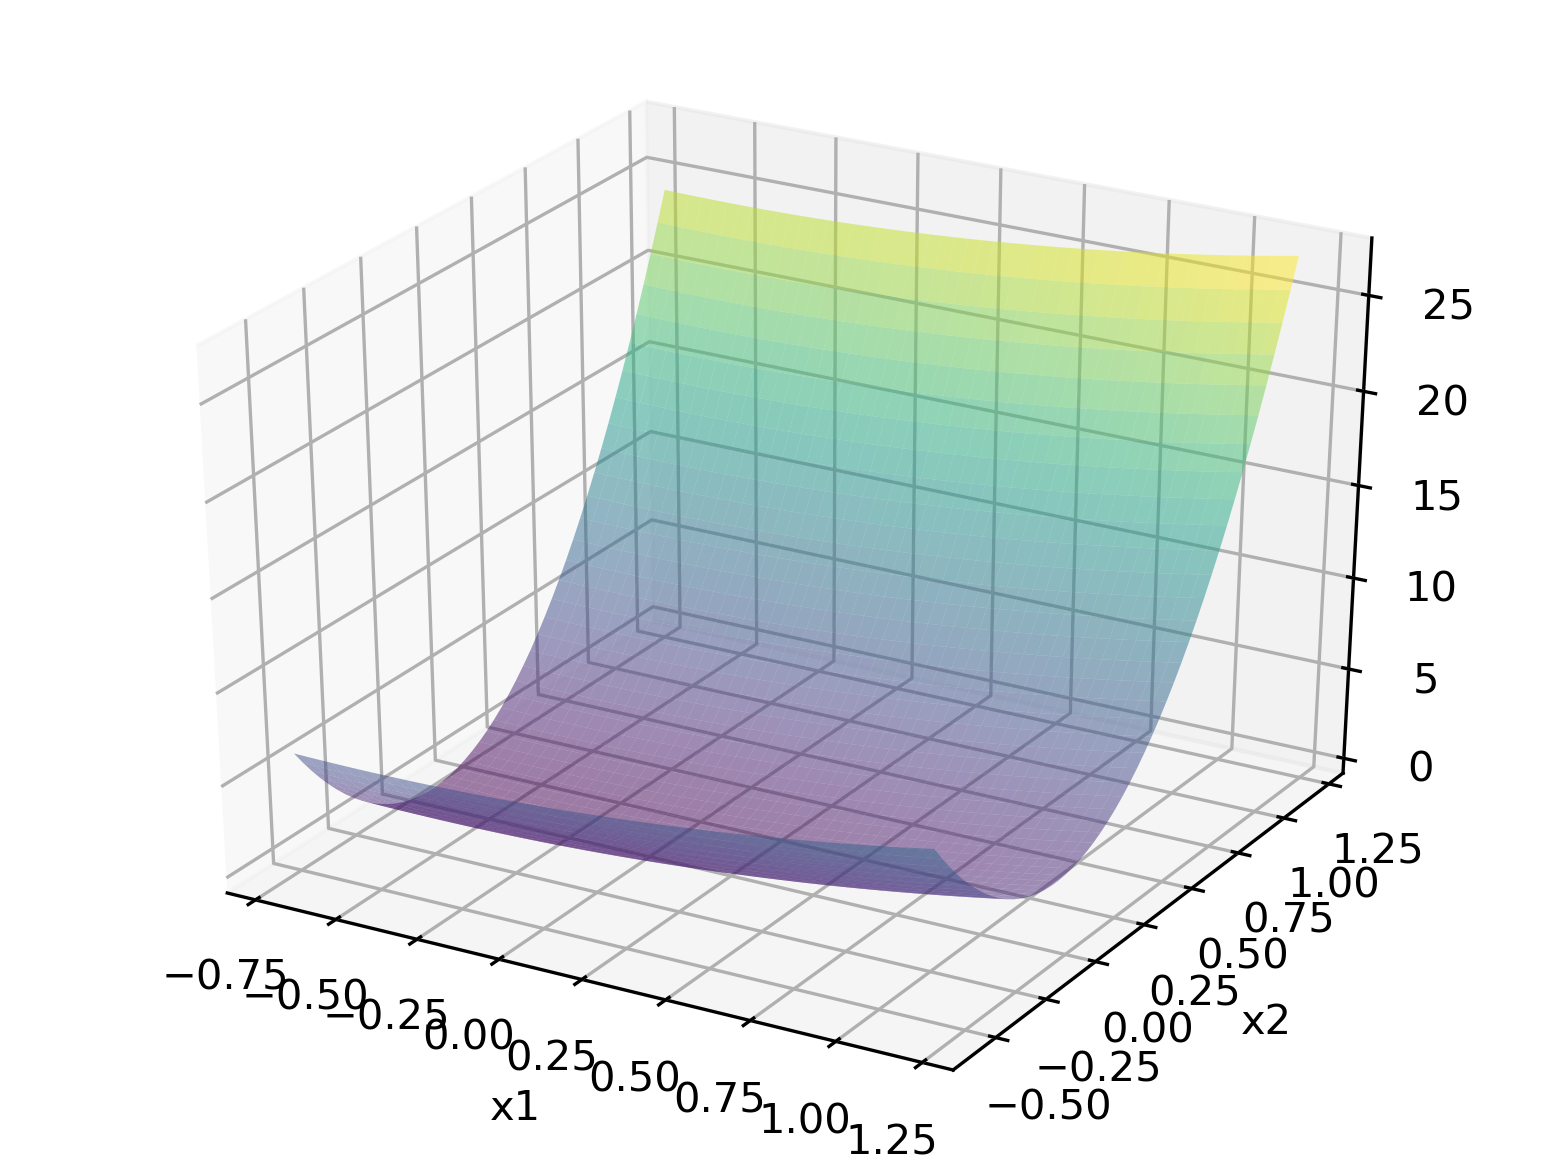
\includegraphics[scale = 0.6]{surface_init.png} &
        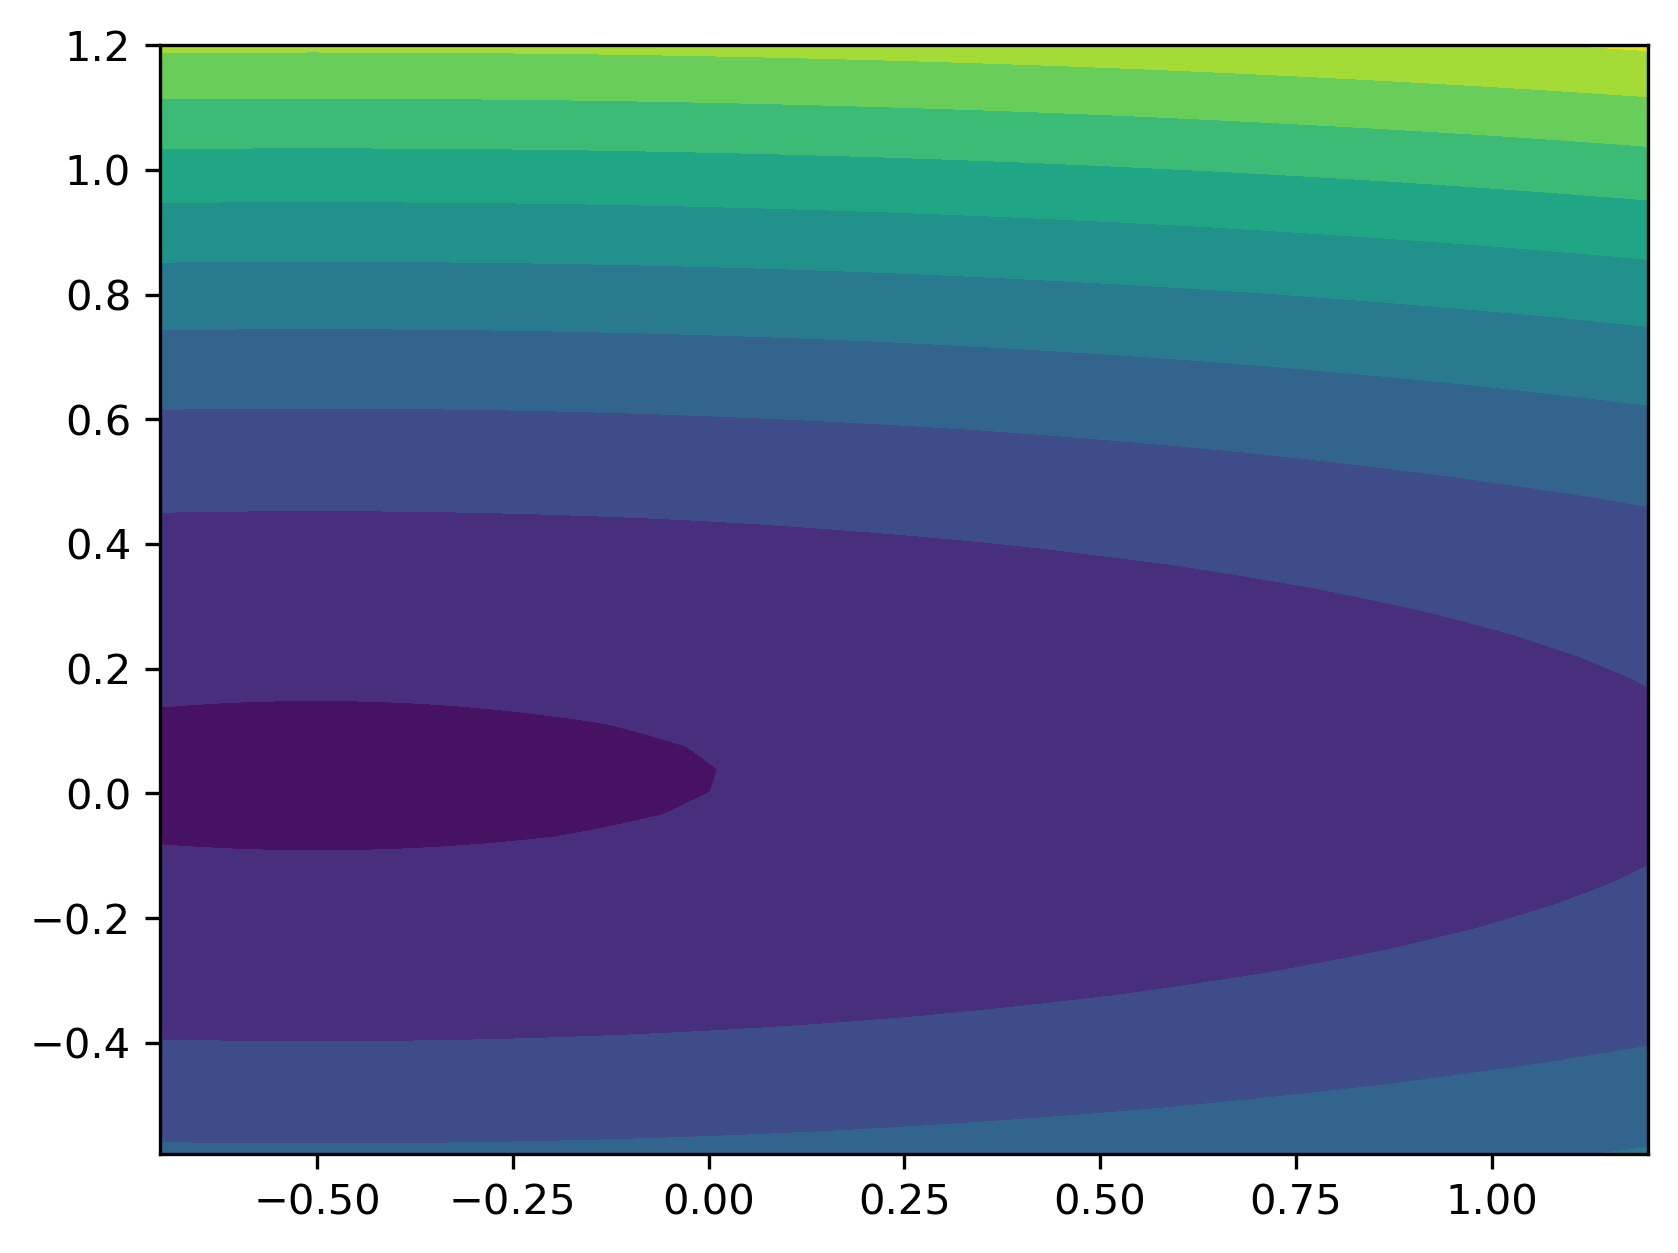
\includegraphics[scale = 0.5]{contour_init.png}
    \end{tabular}
\end{center}
Знайдемо точку мінімуму аналітично:
\begin{gather*}
    \begin{cases}
        f'_x(x,y) = 2x + 0.01y + 1 = 0 \\
        f'_y(x,y) = 36y + 0.01x - 1 = 0
    \end{cases} \Leftrightarrow
    \begin{pmatrix}
        2 & 0.01 \\
        0.01 & 36
    \end{pmatrix}
    \begin{pmatrix}
        x \\
        y
    \end{pmatrix} = 
    \begin{pmatrix}
        -1 \\
        1
    \end{pmatrix} \\
    A = \begin{pmatrix}
        2 & 0.01 \\
        0.01 & 36
    \end{pmatrix},
    \det{A} = 72 - 10^{-4} = 71.9999, A^{-1} = \frac{1}{\det{A}}
    \begin{pmatrix}
        36 & -0.01 \\
        -0.01 & 2
    \end{pmatrix} \\
    \begin{pmatrix}
        x \\
        y
    \end{pmatrix} = A^{-1} \begin{pmatrix}
        -1 \\
        1
    \end{pmatrix} = \frac{1}{71.9999} 
    \begin{pmatrix}
        -36.01 \\
        2.01
    \end{pmatrix} \approx
    \begin{pmatrix}
        -0.50014 \\
        0.0279167
    \end{pmatrix}
\end{gather*}
Для чисельного розв'язання задачі реалізовано метод дроблення кроку та метод найшвидшого спуску для квадратичної функції.
\begin{center}
    \begin{tabular}{|c|c|c|}
        \hline
        {} & \multicolumn{2}{c|}{кількість ітерацій}\\
        \hline
        $x_0$ & {метод дроблення кроку} & {метод найшвидшого спуску}\\
        \hline
        $(-0.5, 0.0028)$ & 7 & 2 \\
        \hline
        $(0, 0)$ & 45 & 79 \\
        \hline
        $(1, 1)$ & 53 & 12 \\
        \hline
        $(10, 10)$ & 60 & 10 \\
        \hline
        $(100, 100)$ & 68 & 12 \\
        \hline
        $(1000, 1000)$ & 81 & 14 \\
        \hline
    \end{tabular}
\end{center}
Відповідні графіки з траєкторіями руху методів до точки мінімуму:
\begin{center}
    Метод дроблення кроку

    \begin{tabular}{c c}
        \includegraphics[scale = 0.55]{result_(-0.5, 0.028)_frac.png} &
        \includegraphics[scale = 0.55]{result_(0, 0)_frac.png} \\
        \includegraphics[scale = 0.55]{result_(1, 1)_frac.png} &
        \includegraphics[scale = 0.55]{result_(10, 10)_frac.png} \\
        \includegraphics[scale = 0.55]{result_(100, 100)_frac.png} &
        \includegraphics[scale = 0.55]{result_(1000, 1000)_frac.png}
    \end{tabular}
\end{center}
\newpage
\begin{center}
    Метод найшвидшого спуску

    \begin{tabular}{c c}
        \includegraphics[scale = 0.55]{result_(-0.5, 0.028)_quad.png} &
        \includegraphics[scale = 0.55]{result_(0, 0)_quad.png} \\
        \includegraphics[scale = 0.55]{result_(1, 1)_quad.png} &
        \includegraphics[scale = 0.55]{result_(10, 10)_quad.png} \\
        \includegraphics[scale = 0.55]{result_(100, 100)_quad.png} &
        \includegraphics[scale = 0.55]{result_(1000, 1000)_quad.png}
    \end{tabular}
\end{center}
\newpage
Перевіримо роботу градієнтного методу з дробленням кроку на тестовій функції 
$f(x, y) = (y-x^2)^2 + (1-x)^2$, що має мінімум в точці $(1, 1)$.
\begin{center}
    \includegraphics[scale = 0.7]{rosenbrok_2.png} \\
    \includegraphics[scale = 0.7]{rosenbrok_5.png} \\
    \includegraphics[scale = 0.7]{rosenbrok_10.png}
\end{center}
\noindent\textbf{Лістинг.}
Текст програми було розділено на \texttt{Optimizer.py} з реалізацією
власне градієнтного методу та \texttt{lab1.py}, де задаються цільові функції.

\noindent\texttt{Optimizer.py}
\lstinputlisting[language = Python, style = python_code]{../code/Optimizer.py}

\noindent\texttt{lab1.py}
\lstinputlisting[language = Python, style = python_code]{../code/lab1.py}

\noindent\textbf{Висновки.} При виконанні даної роботи ми дослідили
застосування градієнтного методу до мінімізації заданої квадратичної функції.
Для пришвидшення збіжності
було реалізовано метод дроблення кроку та метод найшвидшого спуску. Також було порівняно
кількість ітерацій для збіжності методу з різних початкових точок. Метод найшвидшого спуску, цілком очікувано,
збігався за меншу кількість ітерацій, ніж метод дроблення кроку.
\end{document}